\documentclass{standalone}
\usepackage{pgf}
\usepackage{amsmath}
\usepackage{tikz}
\usetikzlibrary{shapes,arrows}
\usetikzlibrary{positioning}
\usepackage{tikz}
\usetikzlibrary{positioning}
\usetikzlibrary{shapes.geometric}
\usetikzlibrary{shapes.misc}
\usepackage{amsmath}
\usepackage{amssymb}
\usepackage{xstring}

\begin{document}
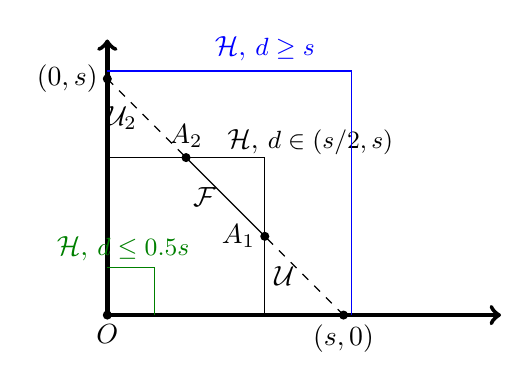
\begin{tikzpicture}
\tikzstyle{myarrow}=[ultra thick,draw=black,->];

\draw [myarrow] (0,0) -- (5,0); % x axis
\draw [myarrow] (0,0) -- (0,3.5) ; % y axis

\draw [fill=black] (0,-0.) circle (0.05) node[below, black]{$O$};
 
\def \slack{3}; 
\draw [fill=black] (\slack,-0.) circle (0.05) node[below, black]{$(s,0)$};
\draw [fill=black] (0,\slack) circle (0.05) node[left, black]{$(0,s)$};

\draw [fill=black] (1.5,1.5)  node[left, black]{$\mathcal{F}$};
\draw [fill=black] (2.5,.5)  node[left, black]{$\mathcal{U}$};
\draw [fill=black] (.5,2.5)  node[left, black]{$\mathcal{U}_2$};

\draw[dashed] (\slack,0) -- (2,1);
\draw [fill=black] (2,1) circle (0.05) node[left, black]{$A_1$};

\draw[dashed]  (0,\slack) -- (1,2);
\draw [fill=black] (1,2) circle (0.05) node[above, black]{$A_2$};

\draw (2,1) -- (1,2);

\colorlet{darkgreen}{green!50!black};
\def \smalld{.6};
\draw[darkgreen] (\smalld,0) -- (\smalld,\smalld) -- (0,\smalld);
\draw [color=blue] (0.2,0.57)  node[above, black]{$\color{darkgreen} \mathcal{H},$ \small $\color{darkgreen}d \leq 0.5s$ \normalsize};


\def \medd{2.0};
\draw (\medd,0) -- (\medd,\medd) -- (0,\medd);
\draw [color=blue] (1.4,2.2)  node[right, black]{$\mathcal{H},$ \small $d\in (s/2,s)$ \normalsize};


\def \larged{3.1};
\draw[blue] (\larged,0) -- (\larged,\larged) -- (0,\larged);
\draw [color=blue] (2,3.1)  node[above, black]{$\color{blue} \mathcal{H},$ \small $\color{blue} d \geq s$ \normalsize};


\end{tikzpicture}
\end{document}



